% ---------------------------------------------------------------------------- %
\chapter{Results}
\label{chap:results}
% ---------------------------------------------------------------------------- %


\begin{itemize}\tightlist
    \item
        Saturation: Lower boundary: bitstream without any input signal
    \item
        Saturation: Upper boundary: Find meaningful equivalent to "no input" at lower boundary
    %\item
    %    Why do we perform DC measurements? (linearity, offset)
    %\item
    %    Why do we  perform AC measurements w/ harmonics? (What  sort of system
    %    can be measured with this chip, how fast is the plant?)
    %\item
    %    Why do we perform SNR measurements?
    \item
        What are potential  measurements which might be of  interest but which
        we  could  not perform  (and  the  reasons  for  which they  were  not
        performed)?
    \item
        What would need to be done to be able to perform those measurements?
    %\item
    %    What kind of measurements were \emph{not} performed, and why?
    %\item
    %    Which measurements were performed?
    %\item
    %    Why are these measurements relevant?
    %\item
    %    What kind of results are we expecting? (Simulation results)
    %\item
    %    What are our actual results?
    %\item
    %    What are potential causes for the differences? (Potentially split this off
    %    into a separate chapter titled \emph{Analysis} or something similar.)
\end{itemize}

%\todo[inline]{Statistical analysis of results}

% --------------------------------------------------------------------------- %
\section{Pre-Amplifier: DC Measurements}
\label{sec:preAmpDC}
% --------------------------------------------------------------------------- %

The preamplifier was directly  measured, isolated from the \sdm, by applying a
number of constant voltages on the input and recording the output voltage with
an oscilloscope on the \signal{TEST OUT} pin.

Since the  preamp  uses  a  switching  capacitor  implementation,  the  output
waveform is of  course  a  square  wave  of  sorts,  as  can be seen in figure
\ref{fig:preamp_waveform}.

\begin{figure}
    \centering
    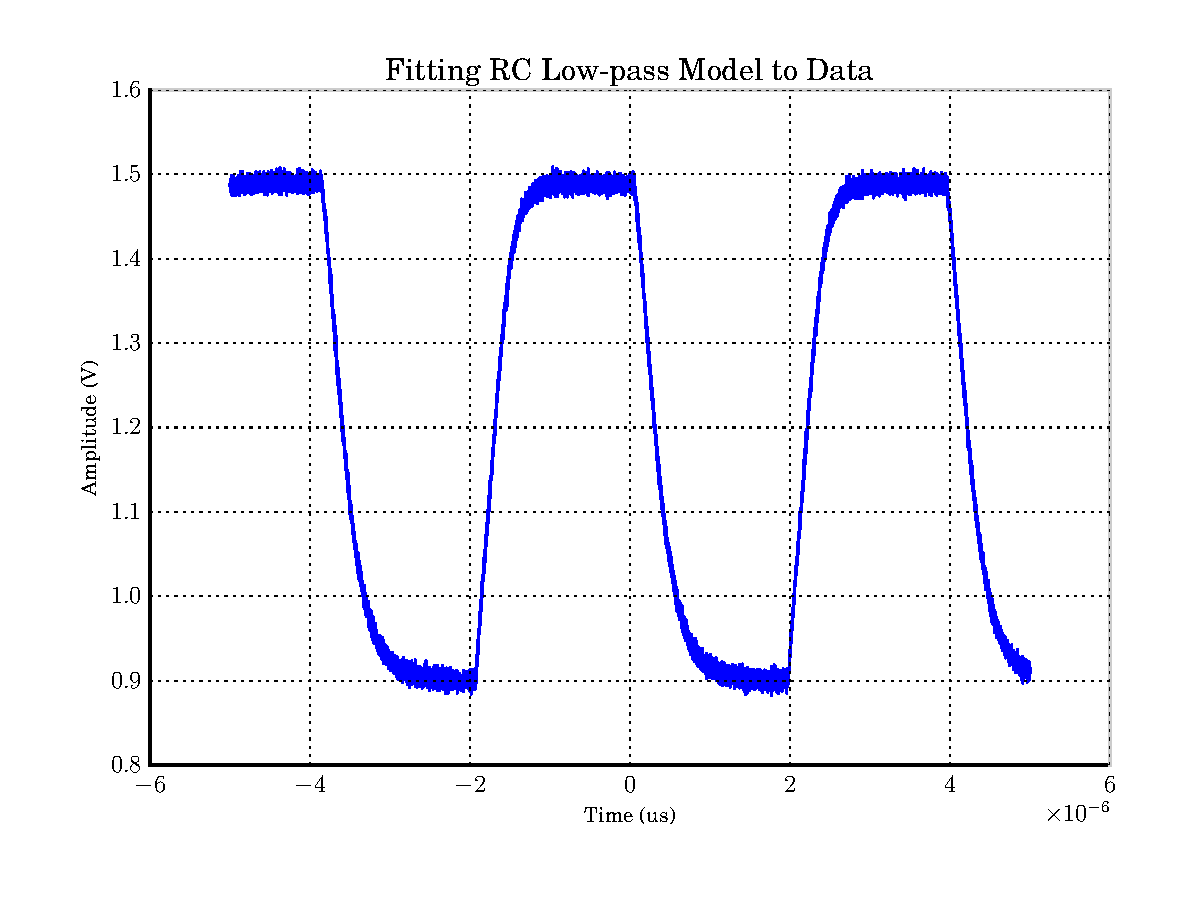
\includegraphics[width=.7\linewidth]{images/plots/preamp_waveform.pdf}
    \caption{Typical preamp output signal as measured on the \signal{TEST OUT} pin.}
    \label{fig:preamp_waveform}
\end{figure}

A first observation to make are the slow rise and fall-times. Indeed,  this is
one  of the major limiting factors of the chip's performance;  If  the  target
voltage can't be reached within half of the clock period (before it  is  reset
again),  the  \sdm will end up  converting  a  lower  voltage  than  expected.

For  every  chip,  for  every sampling frequency, for every gain, inverted and
non-inverted,  11  different  input voltages were applied and the  output  was
measured.  All  of  the  data  was  then fitted using a simple first order  RC
low-pass charge/discharge model, described by the following python code:

\begin{minted}{python}
def preamp_curve(t, amp, amp_offset, period, t_offset, duty_cycle, tau1, tau2):
    def discharge_segment(t, amp, tau):
        return amp * np.exp(-t / tau)
    def charge_segment(t, amp, tau):
        return amp * (1.0 - np.exp(-t / tau))
    t_local = (t+t_offset) % period
    t_switch = period * duty_cycle
    def preamp_curve_single():
        for t_value in t_local:
            if t_value < t_switch:
                yield charge_segment(t_value, amp, tau1) + amp_offset
            else:
                yield discharge_segment(t_value - t_switch, amp, tau2) + amp_offset
    return np.array([x for x in preamp_curve_single()])
\end{minted}

The initial parameters for the  fit  were obtained by first smoothing the data
(using  a  Savitzky-Golay  filter) and finding  the  transition  points.  This
process is illustrated  in  figure  \ref{fig:transition_detection}.  This  was
necessary because there are a lot of local minima the fit could fall into. The
initial period, duty cycle, and phase shift can be extracted from the distance
between the  transition  lines.  The  initial  amplitude  and  offset  can  be
determined with a min/max search.

\begin{figure}
    \centering
    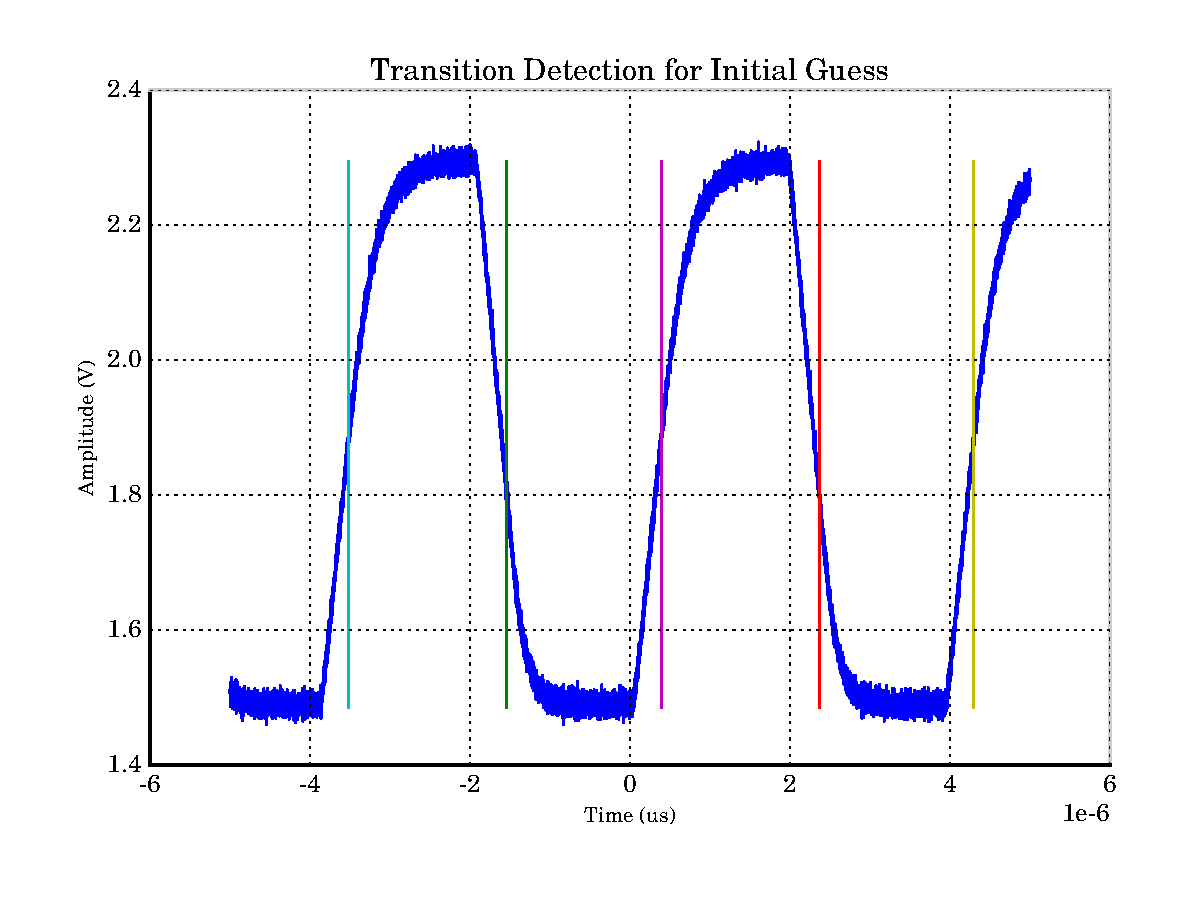
\includegraphics[width=.7\linewidth]{images/plots/transition-detection.pdf}
    \caption{Finding the transition points as a method to accurately estimate initial parameters for duty cycle, period and phase.}
    \label{fig:transition_detection}
\end{figure}

The  most  interesting  parameters  yielded  from  the fit  are  $\Tau_1$  and
$\Tau_2$, which give us a rough idea of the transconductance $g_m$ of the OTA.
The gain can also be easily extracted after  the  fit  by performing a min/max
search   on   the   fitted   curve.   This    is    illustrated    in   figure
\ref{fig:fitting_rc_model} as the horizontal line.

\begin{figure}
    \centering
    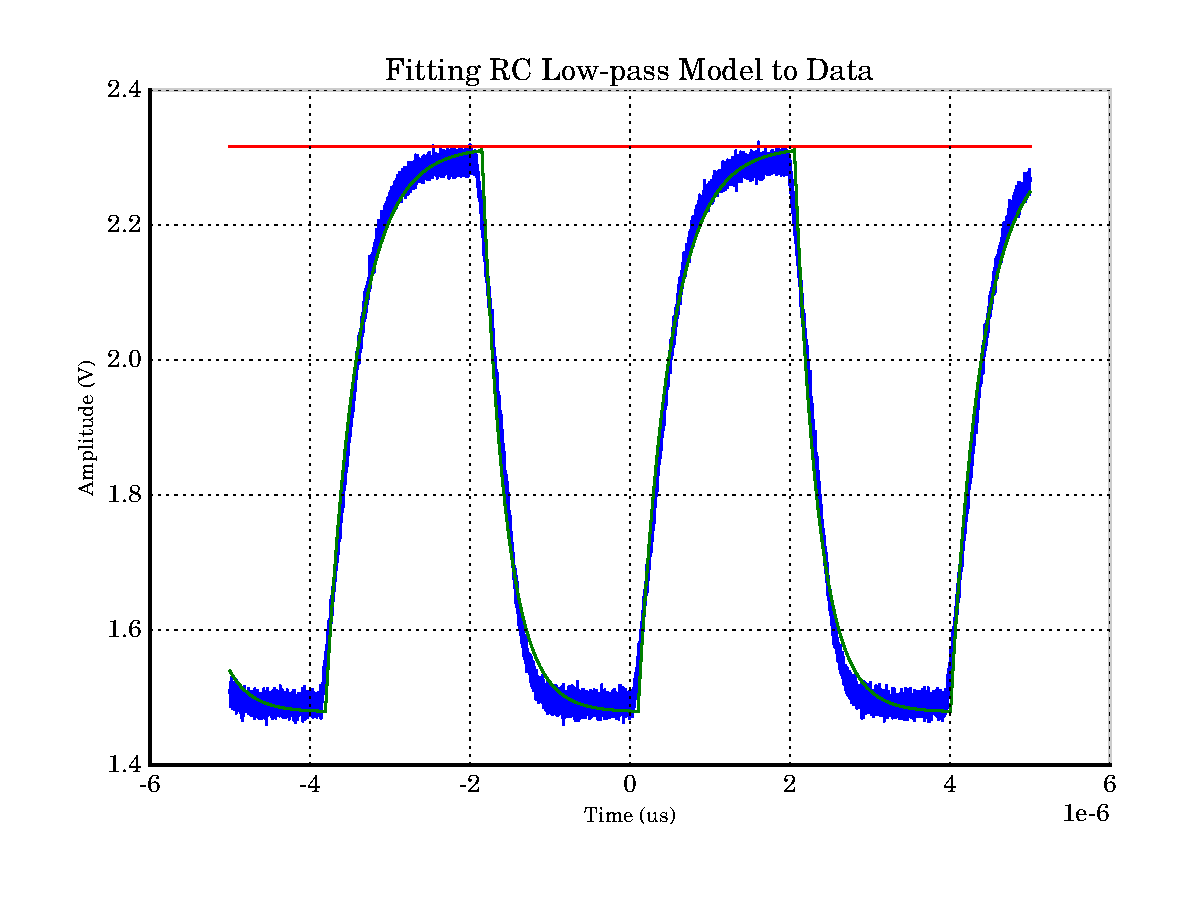
\includegraphics[with=.7\linewidth]{images/fitting_rc_model.pdf}
    \caption{Fitting the RC model to the raw data and determining the preamp output voltage.}
    \label{fig:fitting_rc_model}
\end{figure}

It can be observed that the transconductance $g_m$ is largest  when  near  the
reference voltage $V_{ref}=\SI{1.5}{\volt}$ and  decreases  with  higher input
amplitudes. This effect can be seen in  figure \todo[inline]{generate a figure
with 11 overlapping preamp  signals}. Furthermore, in the same figure, one can
observe slewing on  the  larger  signals. This effect could be included in the
fit model above in future evaluations.

By combining the individual $\Tau$ constants and  plotting them in function of
the input voltage, we see the  effect of $g_m$ decreasing more clearly (figure
\todo[inline]{generate tau  figures}).  Here,  the  results from 10 chips were
statistically averaged to get a better result.

The $\Tau$ constants  appear to be frequency dependent. This doesn't make much
sense and is very likely a direct  result  of  using a very rough model to fit
the data.

By  plotting  the output voltage from the preamp  in  function  of  the  input
voltage and fitting a linear function $y=mx+q$ to the data, we expect a linear
function who's  incline is equal to that of the configured gain. Additionally,
there  we expect a small offset to exist, due to the imperfections of reality.
This  process  is  visualised  in  figure \todo[inline]{generate this figure}.

The  left  column of figure \todo[inline]{generate this}  shows  all  positive
gains (1, 2, 4, 8, 16) for every chip (x  axis)  in  function  of  $fs$. There
appeared to be a  correlation  between sampling frequency $fs$ and gain, which
made  sense  at the time, since at higher sampling frequencies, the output  of
the preamp no longer manages to properly reach the target voltage in time. The
right column of figure \todo[inline]{same figure} shows  the  gain in function
of  sampling  frequency.

It is interesting that as the configurable gain is increased, the measurements
with a higher sampling frequency decrease in expected gain. There is currently
no  explanation  as  to  why  this  is  the  case,  it   is  open  to  further
investigation.

Another interesting observation is what happens when the gain is inverted. The
same  measurements  but   for   negative   gains   can   be   seen  in  figure
\todo[inline]{generate this}. This is much more  what  we  expect  to see: The
sampling frequency and the gain have no significant influence. It is currently
unclear  why  the  preamp  behaves  more correct when  in  inverted  mode.  An
asymmetry  was  also observed while performing the measurements  in  the  lab.

% --------------------------------------------------------------------------- %
\section{Sigma-Delta Converter: DC Measurements}
\label{sec:sigdelDC}
% --------------------------------------------------------------------------- %

The \sdm was measured directly, isolated from the preamp, by applying a number
of  constant  DC  voltages  to  the \signal{TEST OUT} pin  and  recording  the
resulting bit streams using the GPIO \raspi.

Following  the  same  principles as with the pre-amplifier, for every chip and
for every sampling frequency, 11 different input voltages were applied and the
output bit  stream  was  recorded.  All of the data was then evaluated using a
third order sinc-decimation filter to reconstruct a  digital  version  of  the
measured voltage.

By  fitting the linear function $y=mx+q$ to the 11 input/output  voltage  data
points, we expect  to  obtain  a  line  who's incline is equal to 1 and offset
equal  to  0.  In  figure  \todo[inline]{thing} each incline of each  chip  is
plotted for each sampling frequency $fs$.  Similarly,  the offset of each chip
is plotted in figure \todo[inline]{sigdel offsets}.

The  results  show that there is no significant deviation  from  the  expected
values.

During processing of the bit stream data, some anomalies were noticed.  Random
spikes would  occur  here and there. See figure \todo[inline]{show examples at
32, 96 and 256 kHz}. The only correlations that could  be  made  were that the
spikes  occurred  more  often  at  higher sampling rates than they do at lower
sampling rates. After analysing the time axis  to  make  sure  the data points
were  equidistantly  spaced,  random  deviations  were  detected.  This  could
possibly   be   a  result  of  using  the  rather   inaccurate   system   call
\textit{gettimeofday()}  for  generating  time  stamps  on  the   \raspi.  The
deviations are large enough to  suggest the possibility that bits went missing
from the bit stream.

% --------------------------------------------------------------------------- %
\section{Complete System: DC Measurements}
\label{sec:systemDC}
% --------------------------------------------------------------------------- %

The  same  measurements  were  performed  on  the complete chip: That is,  the
pre-amplifier and the \sdm were measured together as one.

As expected, the rather imperfect results from the pre-amplifier combined with
the  perfect  results  from the \sdm result in a semi-imperfect system. Figure
\todo[inline]{Show  linearity  of complete system} shows the various gains  of
the complete system and  figure  \todo[inline]{Show offset of complete system}
shows the offset of the complete system.

%\todo[inline]{Data from Oscilloscope}

%\begin{table}
%    \centering
%    \fontfamily{jkpss}\selectfont
%    \caption{DC Measurements}
%    \label{tab:dcMeas}
%    \begin{tabular}{ccc}
%        \toprule
%        {$V_{\textnormal{in}}$ (\si{\volt})} &
%        {$G_{\textnormal{Preamp}}$}          &
%        {$f_{\textnormal{s}}$ (\si{\kilo\hertz})}         \\
%        \midrule
%        0.5 & {1, 2, 4, 6, 8, 16} & {32, 256} \\
%        0.7 & {1, 2, 4, 6, 8, 16} & {32, 256} \\
%        0.9 & {1, 2, 4, 6, 8, 16} & {32, 256} \\
%        1.1 & {1, 2, 4, 6, 8, 16} & {32, 256} \\
%        1.3 & {1, 2, 4, 6, 8, 16} & {32, 256} \\
%        1.5 & {1, 2, 4, 6, 8, 16} & {32, 256} \\
%        1.7 & {1, 2, 4, 6, 8, 16} & {32, 256} \\
%        1.9 & {1, 2, 4, 6, 8, 16} & {32, 256} \\
%        2.1 & {1, 2, 4, 6, 8, 16} & {32, 256} \\
%        2.3 & {1, 2, 4, 6, 8, 16} & {32, 256} \\
%        2.5 & {1, 2, 4, 6, 8, 16} & {32, 256} \\
%        \bottomrule
%    \end{tabular}
%\end{table}
